\subsection{Avoidance Protocols}
\noindent With the presence of telemetry and range detection data from the sensors, and the obstacles classified and their movement tracked by the camera and the neural networks, FORWARD can proceed to generate guidance feedback and motor commands to steer the rollator and to keep the user safe from collisions. Avoidance protocols may take the form of: emergency stop, right or left hand turn, or veering.

\subsubsection{Emergency Stop}
\noindent An emergency stop would take place if a road is detected (> 2 cars detected) or if there is a drop off (cliff). It would also occur when the rollator acceleration increases rapidly, indicating it is fleeing the user down a decline.\\

\subsubsection{Stationary Obstacle}
\noindent A stationary obstacle such as a wall or staircase would require a complete pivot, either preceding or following an emergency stop. The order would depend on the speed of the user and how much margin there is for guidance.\\


\subsubsection{Polite Response to Obstacle in Motion}
\noindent Polite obstacle avoidance is a veering-moded response to moving obstacles, namely people, pets, and vehicles. The inspiration was drawn from real world experiences, where an obstacle will non-intelligently obstruct fluid travel straight ahead. If there is for example, a person walking from left to right (rollator frame of reference) across the camera field of vision, we can track the coordinates of its detection square, and form some abstract calculation of its velocity. We also have some idea of how fast this might be traveling based on other environmental data obtained by the camera; however, methods beyond the scope of this project would likely be required to harness this and improve avoidance strategies. Nevertheless, knowing the direction of travel of the obstacle means FORWARD can veer the user in the opposite direction. Being opposite is paramount because traveling behind the forward path of the obstacle will vastly decrease the chance of collision, and it will not infringe on either party's convenience or safety. The effects of collision for a stationary object are less severe compared to the likes of a running person or God forbid, a car. FORWARD will be able to confidently halt the user from these dangerous situations, and strategically navigate around them in a seamless manner.\\
\begin{figure}[H]
	\centering
	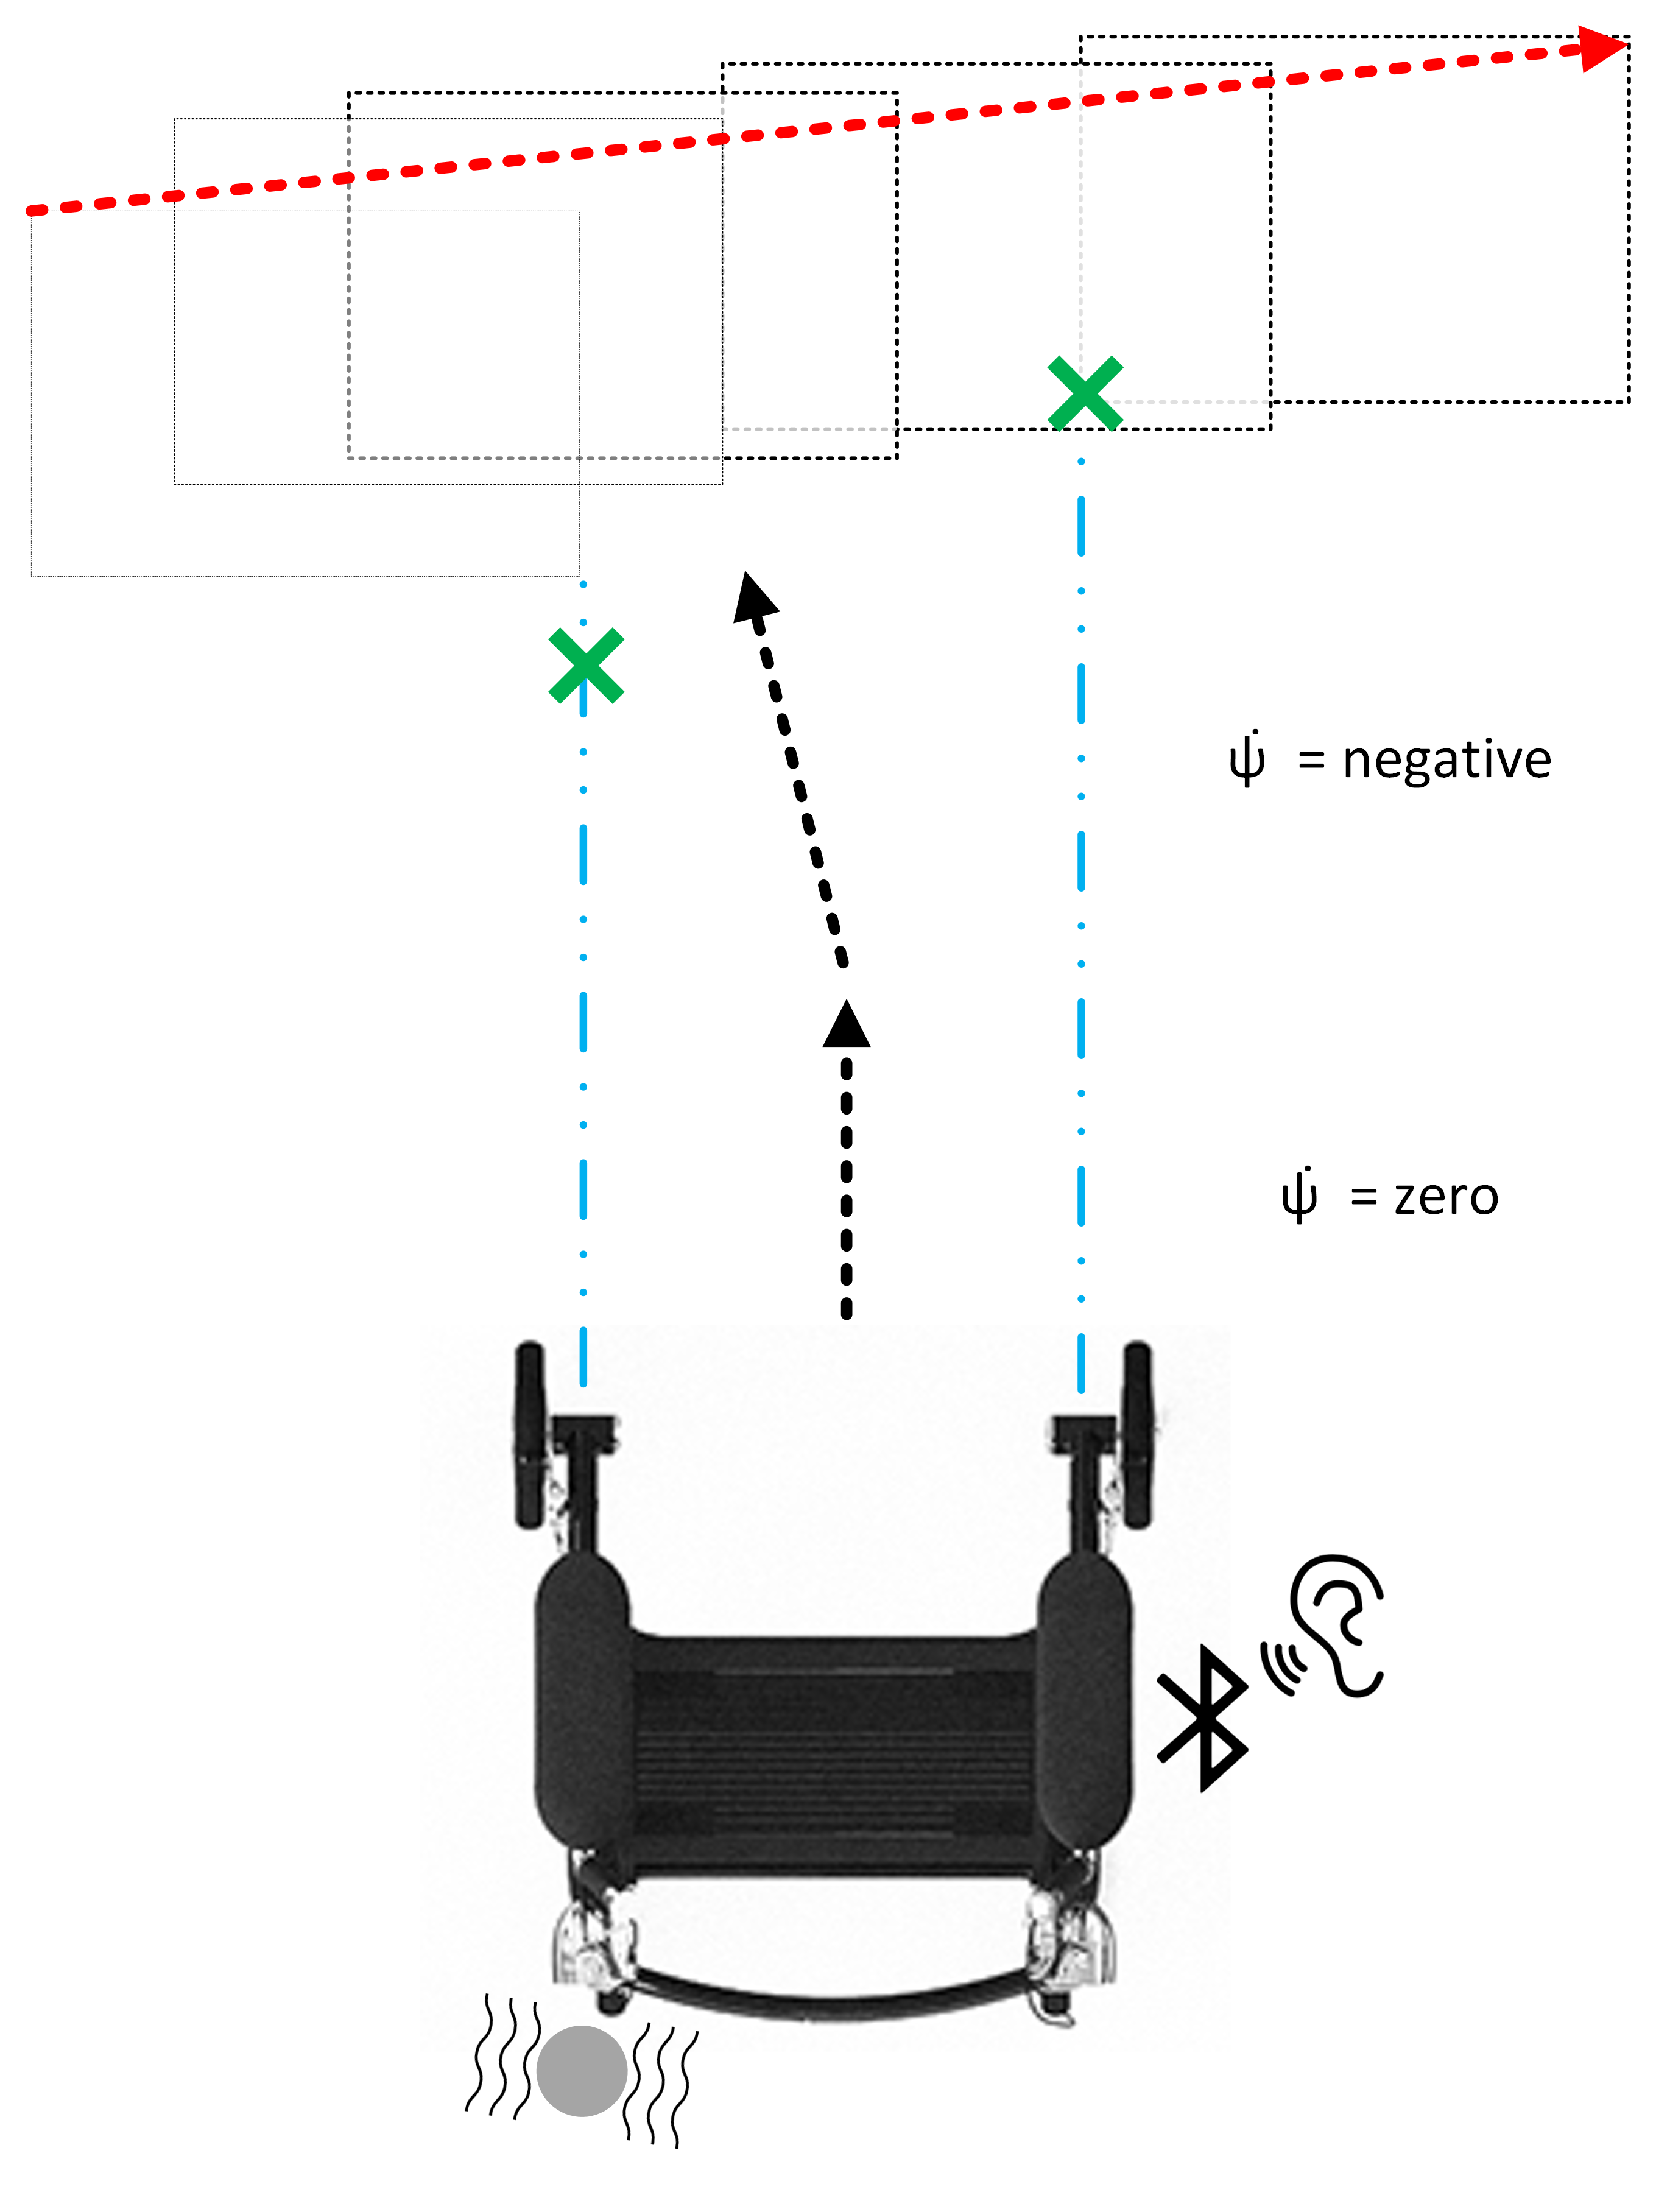
\includegraphics[width=0.8\textwidth]{./Images/Polite-Mobile-Obstacle-Avoidance.png}
	\caption{\label{fig:polite}Polite Obstacle Avoidance}
\end{figure}
